\chapter{Implementation}
\label{chapter:implementation}

\begin{itemize}
  \item intro
  \item Vi lager en liten prototype = ``proof of concept'' -> et begrep vi m\aa~bruke =)
  \item VarRefs m\aa~sendes oppover fra child nodes (ref til tainting deps)
  \item Optimalisering: child nodes vet om de er atomiske/singleton eller ikke
\end{itemize}

\begin{itemize}
  \item Bruk av parseren (den som er generert av antlr osv), XQFTTree-klassen,
  evt. UML
  \item Interfacing av parseren mot oversetteren v\aa r (som oversetter til
  relalg) og UML
  \item Bygging av relasjonsalgebra-tre, UML av operatorklassene
  \item Implementering av visitors
  \item Scoping og symtab (nok en gang..)
  \item hvordan metadata som varrefs og singletonindikering blir sendt oppover
  (Metadata)
  \item Implementering av ``tainting dependencies''
  \item Dataflyt ()
  \item Visible external API
  \item Interface til systemet p\aa~ kommandolinjen
  \item Optimaliseringer, om noen? 
\end{itemize}

\section{Prerequisites}
This proof of concept was implemented in Java 5.0, using regular object
oriented techniques, and is licensed under a liberal BSD license. Instructions
for compilation and installation can be found in TODO: appendix.

\section{Using the XQFT Parser}
The \textit{XQFT Parser}\cite{ourselves} (described in section
\ref{sect:theory:xqftparser}) is a prerequisite for providing the abstract
syntax tree for this XQuery translator. This section will outline how this
parser was used and interfaced with the implementation.

\subsection{Basics and API}
The \textit{XQFT Parser} is a parser generated by the ANTLR parser generator.
Thus, there is a loosely standardised API available for any implementor
utilising a parser generated by ANTLR. In the case of \textit{XQFT Parser}, two
classes are generated: \texttt{XQFTParser} and \texttt{XQFTLexer}. These
classes are used in conjunction on an input string to produce an abstract syntax
tree (see next subsection, and also section
\ref{sect:theory:xqftparser:ast_construction}).

A typical use case to achieve this is shown in figure \ref{}

\begin{figure}[!htp]
\begin{center}
  \begin{Verbatim}
    CharStream cs 
        = new ANTLRStringStream(
            "for $i in (1,2,3) return $i");

    XQFTLexer lexer = new XQFTLexer(cs);

    UnbufferedCommonTokenStream tokens 
        = new UnbufferedCommonTokenStream();
	tokens.setTokenSource(lexer);

    XQFTParser parser = new XQFTParser(tokens);
    parser.setTreeAdaptor(new XQFTTreeAdaptor());
    parser.setLexer(lexer);

    XQFTTree ast = parser.module().getTree();
  \end{Verbatim}
  \caption{Using the XQFTParser and XQFTLexer classes}
  \label{figure:impl:using_xqft}
\end{center}
\end{figure}

\subsection{The XQFTTree class}
\subsection{Interfacing the XQFT Parser}
\section{Constructing the MQL algebra tree}
\label{sect:impl:construct_mql}
The MQL queries are constructed as a tree of operators bottom-up while parsing
the abstract syntax tree (for the corresponding XQuery query). 

\subsection{Operators and parameters}
\begin{figure}[!htp]
\begin{center}
  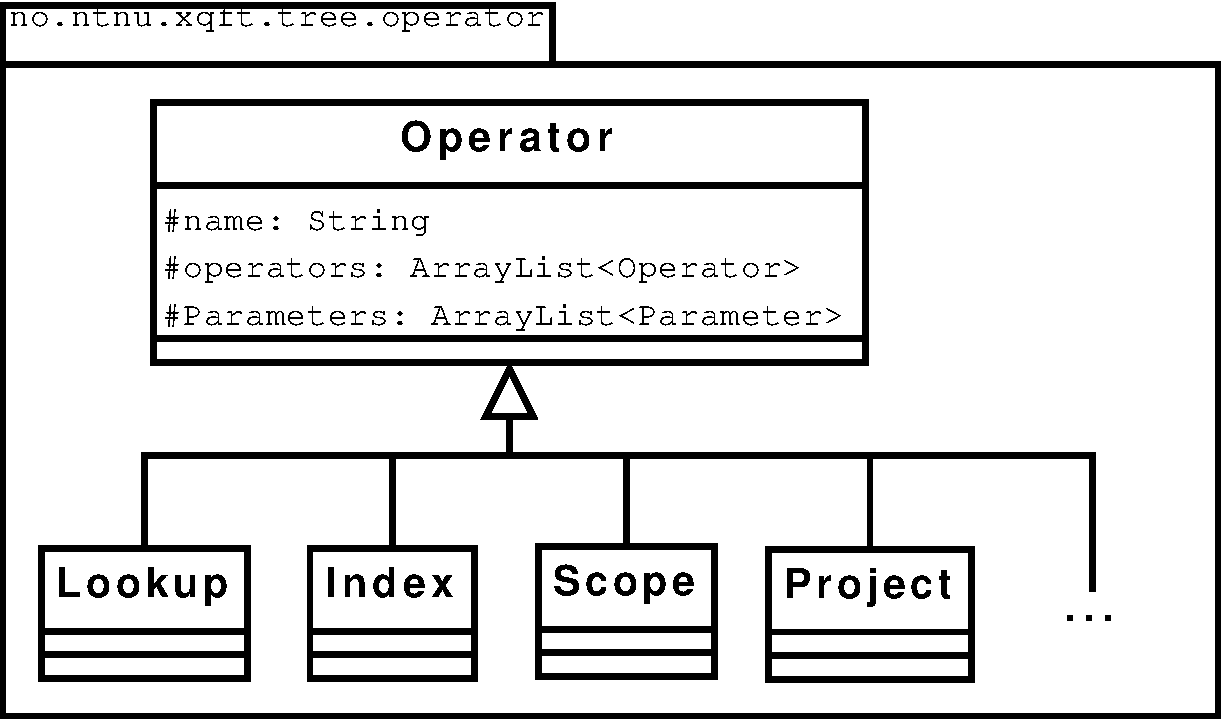
\includegraphics[scale=0.5]{diagrams/mql_operator_uml}
  \caption{Simplified class diagram of MQL operators}
  \label{fig:impl:mql_op_uml}
\end{center}
\end{figure}
The operators modeled in the implementation correspond to the operators
described in section \ref{sect:method:marsOperators}. A simplified class
diagram is shown in figure \ref{fig:impl:mql_op_uml}. Note that the
responsibility with regards to converting an operator to a string
representation is largely left to the various subclasses. However, the default
fallback for the \texttt{Operator} class is to return a string of the form
\begin{Verbatim}
operator_name(param1, param2, ..., paramN; 
              operator1, operator2, ..., operatorM)
\end{Verbatim}
This is sufficient in some cases, such as for the model of the \texttt{cross()}
operator.

\begin{figure}[!htp]
\begin{center}
  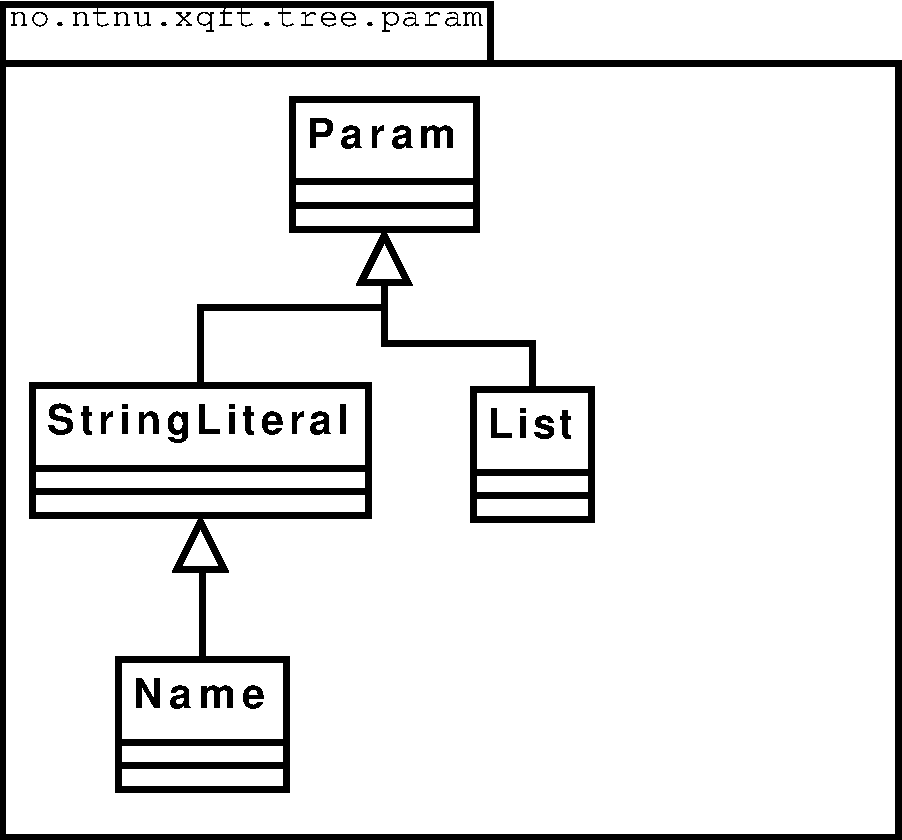
\includegraphics[scale=0.5]{diagrams/mql_param_uml}
  \caption{Class diagram of MQL parameters}
  \label{fig:impl:mql_param_uml}
\end{center}
\end{figure}

MQL parameters (as described in \ref{sect:method:mql:concepts}) are modeled as
seen in figure \ref{fig:impl:mql_param_uml}. Parameters require no complex
structure, and are only created and added to operators as needed.

\subsection{Concepts}
As mentioned, MQL queries are represented as trees, where each node represents
an operator. Each node is an instance of an operator class (as described
above), and contains a list of child operators and a list of parameters. To
convert the operator tree to a MQL query string, simply call the method
\texttt{toPrettyString(0)} on the root node of the operator tree.

\subsection{Usage}
The operator classes are designed to be intuitive and simple to use. Figure
\ref{fig:impl:mql_op_ex1_java} shows one example where a simple operator tree
is built and converted to an MQL query string (the result of which can be seen
in figure \ref{fig:impl:mql_op_ex1_mql}).

%\usepackage{graphics} is needed for \includegraphics
\begin{figure}[htp]
\begin{center}
  \begin{Verbatim}
Lookup lookup = new Lookup("Death in the clouds");
Scope scope = new Scope("/books/book/title", lookup);
Project project = new Project("author", scope);
System.out.println(project.toPrettyString(0));
  \end{Verbatim}
  \caption{Example java code to construct a MQL operator tree}
  \label{fig:impl:mql_op_ex1_java}
\end{center}
\end{figure}

\begin{figure}[htp]
\begin{center}
  \begin{Verbatim}
project([author];
  scope(/books/book/title;
    lookup("Death in the clouds")))
  \end{Verbatim}
  \caption{Resulting MQL query string from example in figure
  \ref{fig:impl:mql_op_ex1_java}}
  \label{fig:impl:mql_op_ex1_mql}
\end{center}
\end{figure}

\section{Context-sensitive visitor}
\label{sect:impl:context_sens_visitor}
In section \ref{sect:theory:parser:tree_parsing} a number of techniques for
tree parsing were presented. In section \ref{sect:method:tree_parsing} the
\textit{context-sensitive visitor pattern} was chosen as the technique for this
implementation. This section will detail the implementation of this design
pattern, and how it is used to performed an assortment of tasks.

\subsection{Basics}
The context-sensitive pattern is designed to be flexible and to generate code
with a higher level of maintainability, for which the rationale was presented
in section \ref{sect:theory:contextVisitorPattern}. 

\begin{figure}[htp]
\begin{center}
  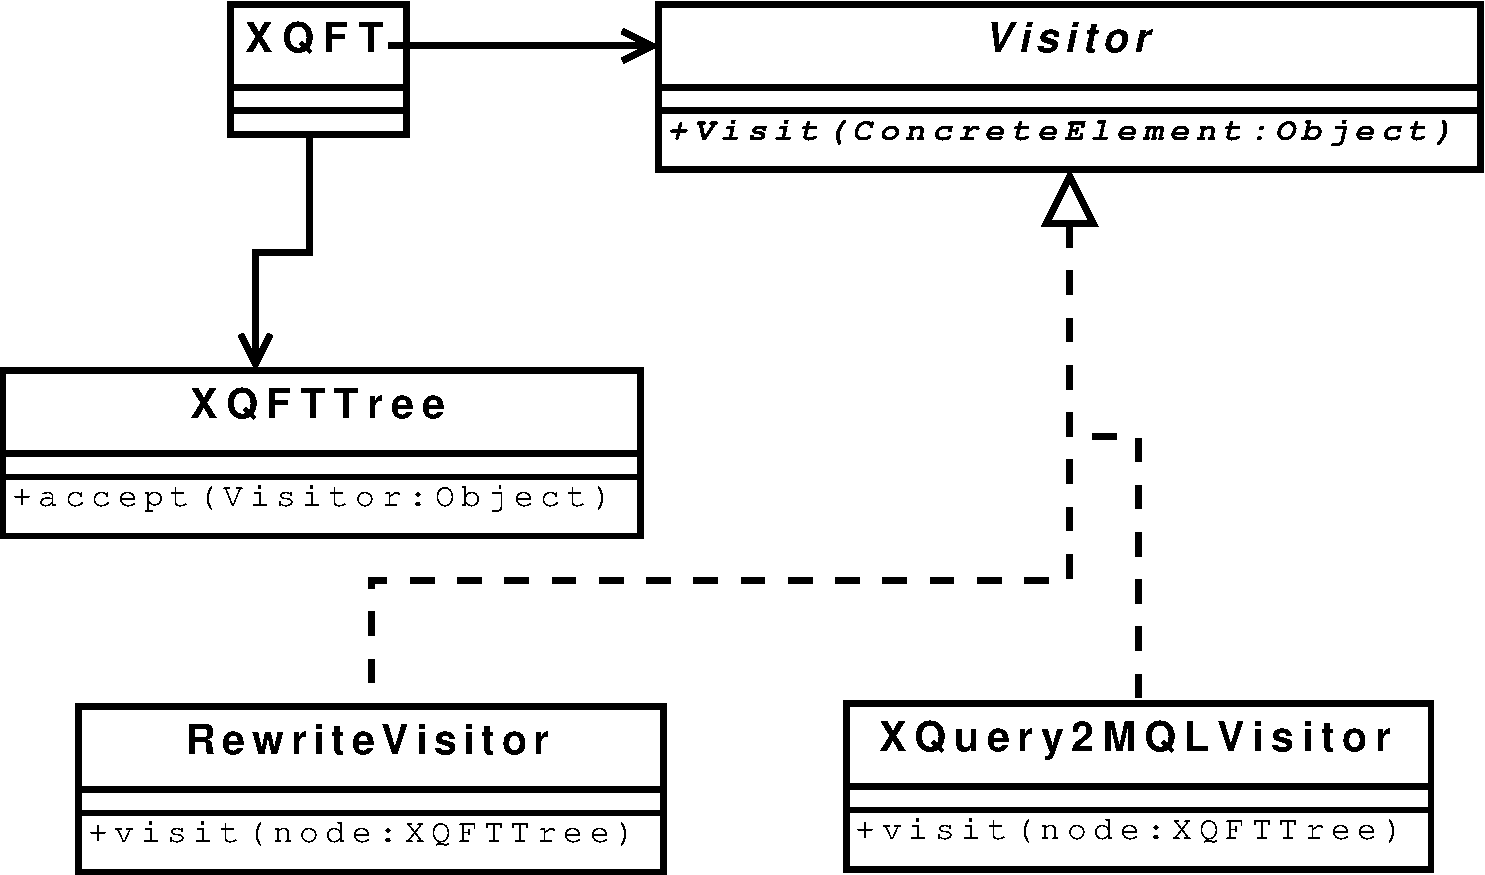
\includegraphics[scale=0.5]{diagrams/context_visitor_pattern_impl}
  \caption{Context sensitive visitor implementation}
  \label{fig:impl:context_sens_visitor_impl}
\end{center}
\end{figure}

The class diagram for the actual implementation of the context-sensitive
visitor pattern can be seen in figure \ref{fig:impl:context_sens_visitor_impl}.
Compare this to the generalized class diagram in figure
\ref{figure:parser:context_visitor_pattern} on page
\pageref{figure:parser:context_visitor_pattern}.

Note that the use of \texttt{XQFTTree} as the element class implies that the
\texttt{XQFTTree} be supplemented with an \texttt{accept()} method to
accommodate this pattern. This method is essentially a static dispatcher which
will call the appropriate method on the visitor based on the token type of the
node currently being visited. Figure \ref{} shows an excerpt of this method and
how it acts on the visitor class.

%\usepackage{graphics} is needed for \includegraphics
\begin{figure}[htp]
\begin{center}
  \begin{Verbatim}	
public TraverseReturn accept(Visitor visitor) {
     case XQFTParser.AST_MODULE:
            return visitor.visitAST_MODULE(this);
        case XQFTParser.AST_FLWOR:
            return visitor.visitAST_FLWOR(this);
        case XQFTParser.AST_FORCLAUSE:
            return visitor.visitAST_FORCLAUSE(this);
        case XQFTParser.AST_LETCLAUSE:
            return visitor.visitAST_LETCLAUSE(this);
        case XQFTParser.AST_ORDERBYCLAUSE:
            return visitor.visitAST_ORDERBYCLAUSE(this);
        case XQFTParser.AST_WHERECLAUSE:
            return visitor.visitAST_WHERECLAUSE(this);
                          .
                          .
                          .
  \end{Verbatim}
  \caption{Excerpt from the accept() method in the XQFT class}
  \label{figureLabel}
\end{center}
\end{figure}

\subsection{The Rewrite visitor}
The \textit{Rewrite visitor} is used to perform rewrite operations on the
abstract syntax tree before performing the actual translation. In particular,
these rewrite operations consists of normalizing the required subtrees of the
syntax tree to a subset of XQuery Core (as described in sections
\ref{sect:theory:xquery:XQcore} and \ref{sect:method:ast_rewrite}).

\subsection{The XQuery2MQL visitor}
The \textit{XQuery2MQL visitor} performs the bulk of the work related to
performing the translation of XQuery to MQL. This visitor is capable of
re-instantiating itself (or other visitors) when entering new contexts, such as
path predicates. 
\section{Scoping and Symbol Tables}
Crucial to the implementation of the Tainting Dependencies (TD) methodology
described in chapter \ref{chapter:translation} is the ability to
maintain a contextual environment with scoping and symbol tables. This section
details the implementation of this, and how it is used to meet the
requirements of TD.

\subsection{Concepts}
The scoping system in the implementation is based on building a scope tree. The
previous scope, if any, is set as parent of the new scope, and the previous
scope maintains a list of child scopes -- this is referred to as
\textit{pushing a scope}. When exiting a scoped subexpression in the AST, the
previous scope is again set as the current scope. This is referred to as
\textit{popping a scope}. A reference to the root scope node is always
maintained. Considering the example XQuery query in figure
\ref{fig:impl:scope_tree_ex_code}, the scope tree in figure
\ref{fig:impl:scope_tree_ex} is generated. The scope itself contains \emph{one}
symbol table for the current scope.

\begin{figure}[!htp]
\begin{center}
\begin{minipage}[h]{9cm}
\begin{verbatim}
for $i in (1,2,3) return 
  for $a in (4,5,for $b in (6,7,8) return $b) 
    return ($i,$a)
\end{verbatim}
  \caption{Scope tree example code}
  \label{fig:impl:scope_tree_ex_code}
  \end{minipage}
\end{center}
\end{figure}

\begin{figure}[!htp]
\begin{center}
  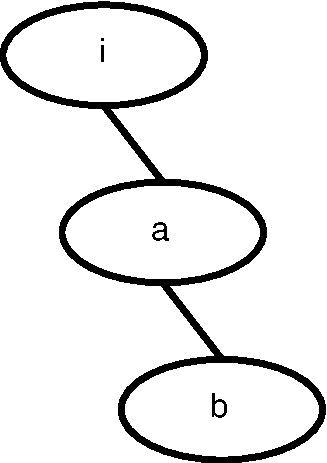
\includegraphics[width=0.2\textwidth]{diagrams/scope_tree_ex}
  \caption{Scope tree for source code in figure
  \ref{fig:impl:scope_tree_ex_code}} 
  \label{fig:impl:scope_tree_ex}
\end{center}
\end{figure}

Entries in the symbol table are represented through an instance of the
\texttt{SymTabEntry} class which maintains metadata about symbols (such as
symbol name, a flag indicating whether it's an iterator variable, and an
evaluated expression). The symbol table is realised as a subclass of the
\texttt{HashMap} class in the \texttt{java.util} package, and is constrained to
storing instances of \texttt{SymTabEntry}, with the symbol name as key.

\subsection{Semantics}
The scoping semantics are encapsulated in a singleton manner in the class
\texttt{Scope}, with static methods available for pushing and popping scopes,
and storing and retrieving symbols. The external (static) API as available to a
user of the scope system is shown in figure \ref{fig:impl:scope_uml}.

\begin{figure}[!htp]
\begin{center}
  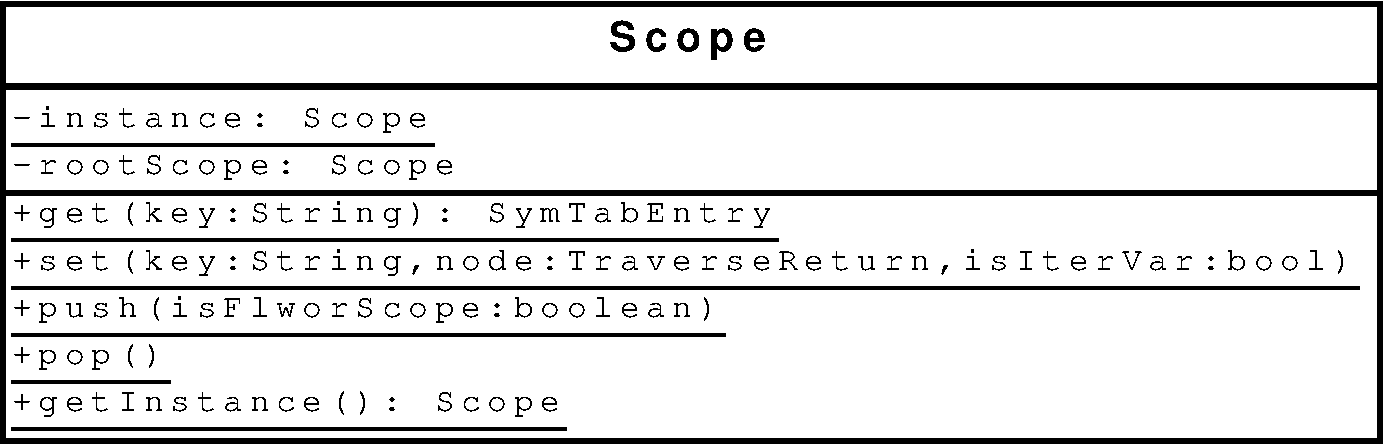
\includegraphics[width=0.7\textwidth]{diagrams/scope_uml}
  \caption{Scope API}
  \label{fig:impl:scope_uml}
\end{center}
\end{figure}

A new scope is \textit{pushed} whenever a \texttt{for}-clause is encountered while
parsing the abstract syntax tree, and the current scope is \textit{popped} after
evaluating a \texttt{return}-clause -- both of which occur within a FLWOR expression.

The scoping system also tracks iteration variables. That is, for any scope,
there is \textit{one and only one} iteration variable, except in the top scope
where there is no iteration variable. The concept of an iteration variable is
explained in definition \ref{def:iterVarDep}. Tracking of these
variables are reviewed in section \ref{sect:impl:tainting_deps}.
\section{Passing Metadata Between Nodes}
To implement the Tainting Dependencies method it is necessary to pass
metadata upwards when parsing the syntax tree, such as
iterator dependencies and flags to indicate singleton nodes (for simplifications). Additionally, the
operator tree which is being built bottom-up (as described earlier in section
\ref{sect:impl:construct_mql}) is also required to be passed upwards. 

This is achieved through the \texttt{TaverseReturn}, which models a return type
when visiting nodes in the syntax tree. That is, the visitor methods are
responsible of 1) visiting any child nodes, and 2) returning an instance of the
\texttt{TraverseReturn} class based on what was returned from the child nodes,
if anything.

\subsection{The TraverseReturn Class}
The class diagram for the \texttt{TraverseReturn} class is shown in figure
\ref{fig:impl:meta:traverse_uml}. Note the flag to indicate if the current
context is a singleton, the reference to an MQL operator tree (which is being
built bottom-up), and a reference to a set of iterator dependencies (in the implementation called
\texttt{varRefs}).

\begin{figure}[!htp]
\begin{center}
  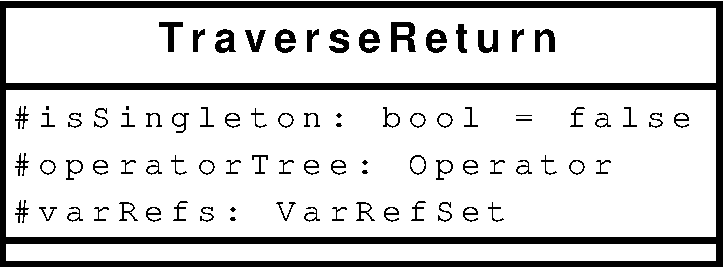
\includegraphics[scale=0.5]{diagrams/traversereturn_uml}
  \caption{TraverseReturn class diagram}
  \label{fig:impl:meta:traverse_uml}
\end{center}
\end{figure}

The \texttt{TraverseReturn} class is, as mentioned, used in the visitor when
visiting nodes in the abstract syntax tree (see section
\ref{sect:impl:context_sens_visitor}). A typical use case is shown in figure
\ref{fig:impl:meta:traverse_usage_ex}, which is an excerpt from the
implementation.

\subsection{Iterator Dependencies}
Iterator dependencies, described in section \ref{sect:trans:TD:basics}, are
passed upwards together with the MQL operator tree being built during the syntax
tree parsing process. These sets of dependencies are handled by th \texttt{VarRef} and \texttt{VarRefSet} classes.
A class diagram for these classes is shown in figure \ref{fig:impl:meta:varrefset_uml}.

\begin{figure}[!htp]
\begin{center}
  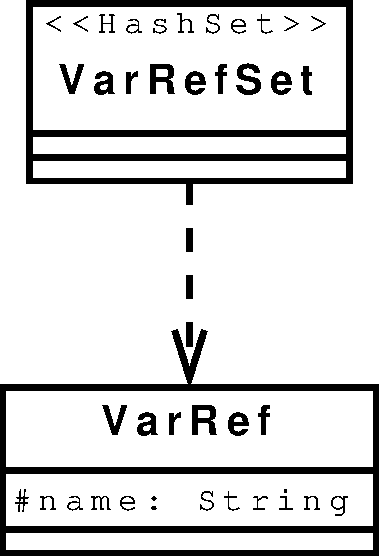
\includegraphics[scale=0.5]{diagrams/varrefset_uml}
  \caption{\texttt{VarRefSet} and \texttt{VarRef} class diagram}
  \label{fig:impl:meta:varrefset_uml}
\end{center}
\end{figure}

As described in section \ref{sect:trans:TD:dependency}, an iterator variable reference is always dependent on
its corresponding iterator. Thus, when a iterator variable is encountered during the parse process, and the
variable is being ``read'' and not assigned or declared, the corresponding iterator is added to the current set of
iterator dependencies. The example in figure \ref{fig:impl:meta:var_ref_ex} shows the variable \texttt{\$a}
being read, in which case the iterator is added to the \texttt{TraverseReturn}
to-be-returned's set of dependencies.

\begin{figure}[!htp]
\begin{center}
\begin{minipage}[h]{5cm}
\begin{verbatim}
for $i in (1,2,3) return 
    ($a,4,5)
\end{verbatim}
\end{minipage}
  \caption{Example of the variable \texttt{\$a} being read. Note that the iterator
  variable \texttt{\$i} is never read}
  \label{fig:impl:meta:var_ref_ex}
\end{center}
\end{figure}

The source code excerpt in figure \ref{fig:impl:meta:var_ref_impl2} shows how
iterator dependencies are treated in the visitor implementation.

\begin{figure}[!htp]
\begin{center}
\begin{Verbatim}
// Fetch entry from symtab
SymTabEntry entry = Scope.get(tree.getChild(0).getText());
            
// Obtain and append new var ref
TraverseReturn tr = entry.getTraverseReturn();
tr.getVarRefs().add(new VarRef(tree.getChild(0).getText()));

return tr;
\end{Verbatim}
  \caption{Appending a new variable reference}
  \label{fig:impl:meta:var_ref_impl2}
\end{center}
\end{figure}

\subsection{Singleton nodes}
Singleton nodes are nodes corresponding to expressions that return a sequence of exactly one item. In
the cases where this is known to be true, the result from a translation can be
tagged with this information and used later to simplify the translation of
sequence construction (as described in section \ref{sect:impl:td:seq}).

This is the case of integer literal nodes as well as iterator variable lookups in the
symbol table. The case of integer literal nodes is shown in figure
\ref{fig:impl:meta:traverse_usage_ex} in the next section. The case of variable
lookups is somewhat less intuitive, since the singleton flag is actually
stored when a variable is first set. That is, the right-hand side of the
assignment is translated once and annotated with the singleton flag, which is
then set for all subsequent lookups in the symbol table. The excerpt in figure 
\ref{fig:impl:meta:var_assign_ex} shows how this is done in the implementation.

\begin{figure}[!htp]
\begin{center}
\begin{Verbatim}
// Visit children on the right side of the assignment
TraverseReturn tr = acceptThis(tree.getChild(1));

// Required for tainting deps method
Project project = new Project("[" + varName + "numb, value]", 
                      tr.getOperatorTree());

// Assign metadata
tr.setOperatorTree(project);
tr.setSingleton(true);

// Enter into symbol table
SymTabEntry tmp = Scope.set(tree.getChild(0).getText(), 
                      tr, isIterationVar);
\end{Verbatim}
  \caption[Iterator variable annontion with singleton flag]{Iterator variable
  assignment example, annotated with the singleton flag before being entered into the symtab}
  \label{fig:impl:meta:var_assign_ex}
\end{center}
\end{figure}

\subsection{Example of usage}
In the example in figure \ref{fig:impl:meta:traverse_usage_ex}, an
integer literal node is visited (a node that simply holds an integer). A
\texttt{make()} MQL operator as well as a new \texttt{TraverseReturn}
instance is created. The \texttt{make()} operator is then appended to the 
\texttt{TraverseReturn} instance, and the \textit{isSingleton} flag is set to 
\textit{true} since the result of this translation is a single item.

\begin{figure}[!htp]
\begin{center}
\begin{Verbatim}
public TraverseReturn visitIntegerLiteral(XQFTTree tree) {

    Make make = new Make("name:=[index, value], [1, " + tree.getText());
    TraverseReturn tr = new TraverseReturn();        
    tr.setSingleton(true);
    tr.setOperatorTree(make);
    return tr;
}
\end{Verbatim}
  \caption{TraverseReturn usage example}
  \label{fig:impl:meta:traverse_usage_ex}
\end{center}
\end{figure}
\section{Tainting dependencies}
``Tainting dependencies'' is a method of translating XQuery queries to
relational algebra. The semantics of this method is described in detail
throughout section \ref{sect:trans:taintingDependencies}. This section
describes an implementation of a subset of this method which is capable of
translating simple FLWOR expressions, sequences, and variables. 

\label{sect:impl:tainting_deps}
Dette blir den lengste seksjonen i dette kapittelet, h\aa per jeg.
\subsection{FLWOR expressions}



\subsection{Sequences}
\label{sect:impl:td:seq}
\begin{itemize}
  \item behandler parantes istf. komma for sekvenser (ref spec) 
\end{itemize}




\section{Data flow}
\begin{itemize}
  \item grammatikk -> antlr -> parser
  \item xquery -> parser -> visitor -> relalg
\end{itemize}

\section{Visible external API}
\begin{itemize}
  \item Vise hvordan oversetteren kan brukes i sin helhet i andre programmer
\end{itemize}

\section{Command line interface}
\marginpar{\underline{\textbf{\Large TODO:}}\scriptsize ha det i appendix ala i fjor?}
Dette er ikke s\aa~veldig viktig \aa~skrive om, men greit \aa~ha med.
\begin{itemize}
  \item Argsengine
  \item Aksepterer flere strenger og filer
  \item Outputter til graphviz/dot og pdf, hvis tilgjengelig
  \item Dependencies (jar-filer og drit)
\end{itemize}

\section{Optimalisations?}

\section{Summary}
\label{sect:impl:summary}
\begin{itemize}
  \item sammendrag av dette kap
\end{itemize}